%%%%%%%%%%%%%%%%%%%%%%%%%%%%%%%%%%%%%
%                                   %
% Compile with XeLaTeX and biber    %
%                                   %
% Questions or comments:            %
%                                   %
% joshua dot mcneill at uga dot edu %
%                                   %
%%%%%%%%%%%%%%%%%%%%%%%%%%%%%%%%%%%%%

\documentclass{beamer}
  % Read in standard preamble (cosmetic stuff)
  %%%%%%%%%%%%%%%%%%%%%%%%%%%%%%%%%%%%%%%%%%%%%%%%%%%%%%%%%%%%%%%%
% This is a standard preamble used in for all slide documents. %
% It basically contains cosmetic settings.                     %
%                                                              %
% Joshua McNeill                                               %
% joshua dot mcneill at uga dot edu                            %
%%%%%%%%%%%%%%%%%%%%%%%%%%%%%%%%%%%%%%%%%%%%%%%%%%%%%%%%%%%%%%%%

% Beamer settings
% \usetheme{Berkeley}
\usetheme{CambridgeUS}
% \usecolortheme{dove}
% \usecolortheme{rose}
\usecolortheme{seagull}
\usefonttheme{professionalfonts}
\usefonttheme{serif}
\setbeamertemplate{bibliography item}{}

% Packages and settings
\usepackage{fontspec}
  \setmainfont{Charis SIL}
\usepackage{hyperref}
  \hypersetup{colorlinks=true,
              allcolors=blue}
\usepackage{graphicx}
  \graphicspath{{../../figures/}}
\usepackage[normalem]{ulem}
\usepackage{enumerate}

% Document information
\author{M. McNeill}
\title[FREN2001]{Français 2001}
\institute{\url{joshua.mcneill@uga.edu}}
\date{}

%% Custom commands
% Lexical items
\newcommand{\lexi}[1]{\textit{#1}}
% Gloss
\newcommand{\gloss}[1]{`#1'}
\newcommand{\tinygloss}[1]{{\tiny`#1'}}
% Orthographic representations
\newcommand{\orth}[1]{$\langle$#1$\rangle$}
% Utterances (pragmatics)
\newcommand{\uttr}[1]{`#1'}
% Sentences (pragmatics)
\newcommand{\sent}[1]{\textit{#1}}
% Base dir for definitions
\newcommand{\defs}{../definitions}


  % Packages and settings

  % Document information
  \subtitle[Transport et \lexi{y}]{Les moyens de transport et le pronom \lexi{y}}

\begin{document}
  % Read in the standard intro slides (title page and table of contents)
  \begin{frame}
    \titlepage
    \tiny{Office: % Basically a variable for office hours location
Gilbert 121\\
          Office hours: % Basically a variable for office hours
 lundi, mercredi, vendredi 10:10--11:10
}
  \end{frame}

  \begin{frame}[t]{Pourquoi voyager}
    \begin{columns}
      \column{0.5\textwidth}
        \small
        Pourquoi est-ce qu'on aller aux endroits suivants? Donnez des suggestions en utilisant le pronom \lexi{y}.
        \begin{enumerate}
          \item Les Kerboul sont allés à la Nouvelle-Orléans.
          \item<2->[$\to$] Ils \alert{y} sont allés pour ...
          \item<3-> Les Dupuis vont aller dans les Alpes.
          \item<4->[$\to$] Ils vont \alert{y} aller pour ...
          \item<5-> Raymond veut aller en Guadeloupe.
          \item<6->[$\to$] Il veut \alert{y} aller pour ...
          \item<7-> Christiane va au Mexique.
          \item<8->[$\to$] Elle \alert{y} va pour ...
        \end{enumerate}
      \column{0.5\textwidth}
        \begin{minipage}[c][0.8\textheight]{\linewidth}
          \begin{center}
            \only<1-2>{
              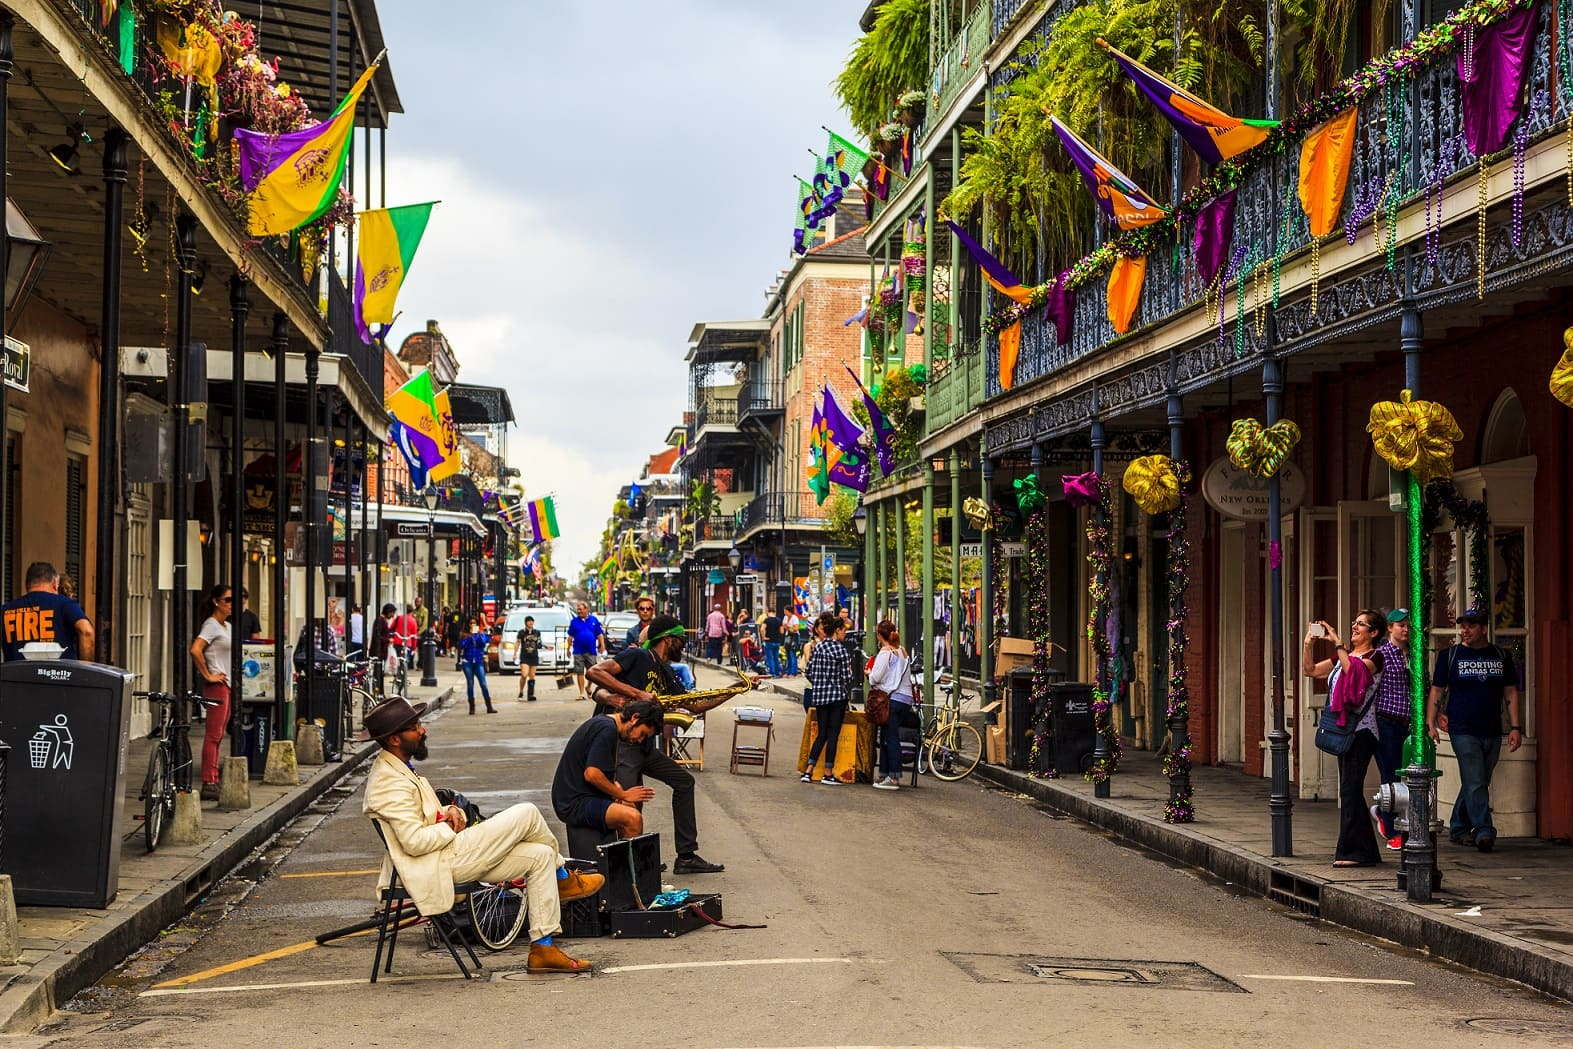
\includegraphics[scale=0.1]{nola.jpg}
            }
            \only<3-4>{
              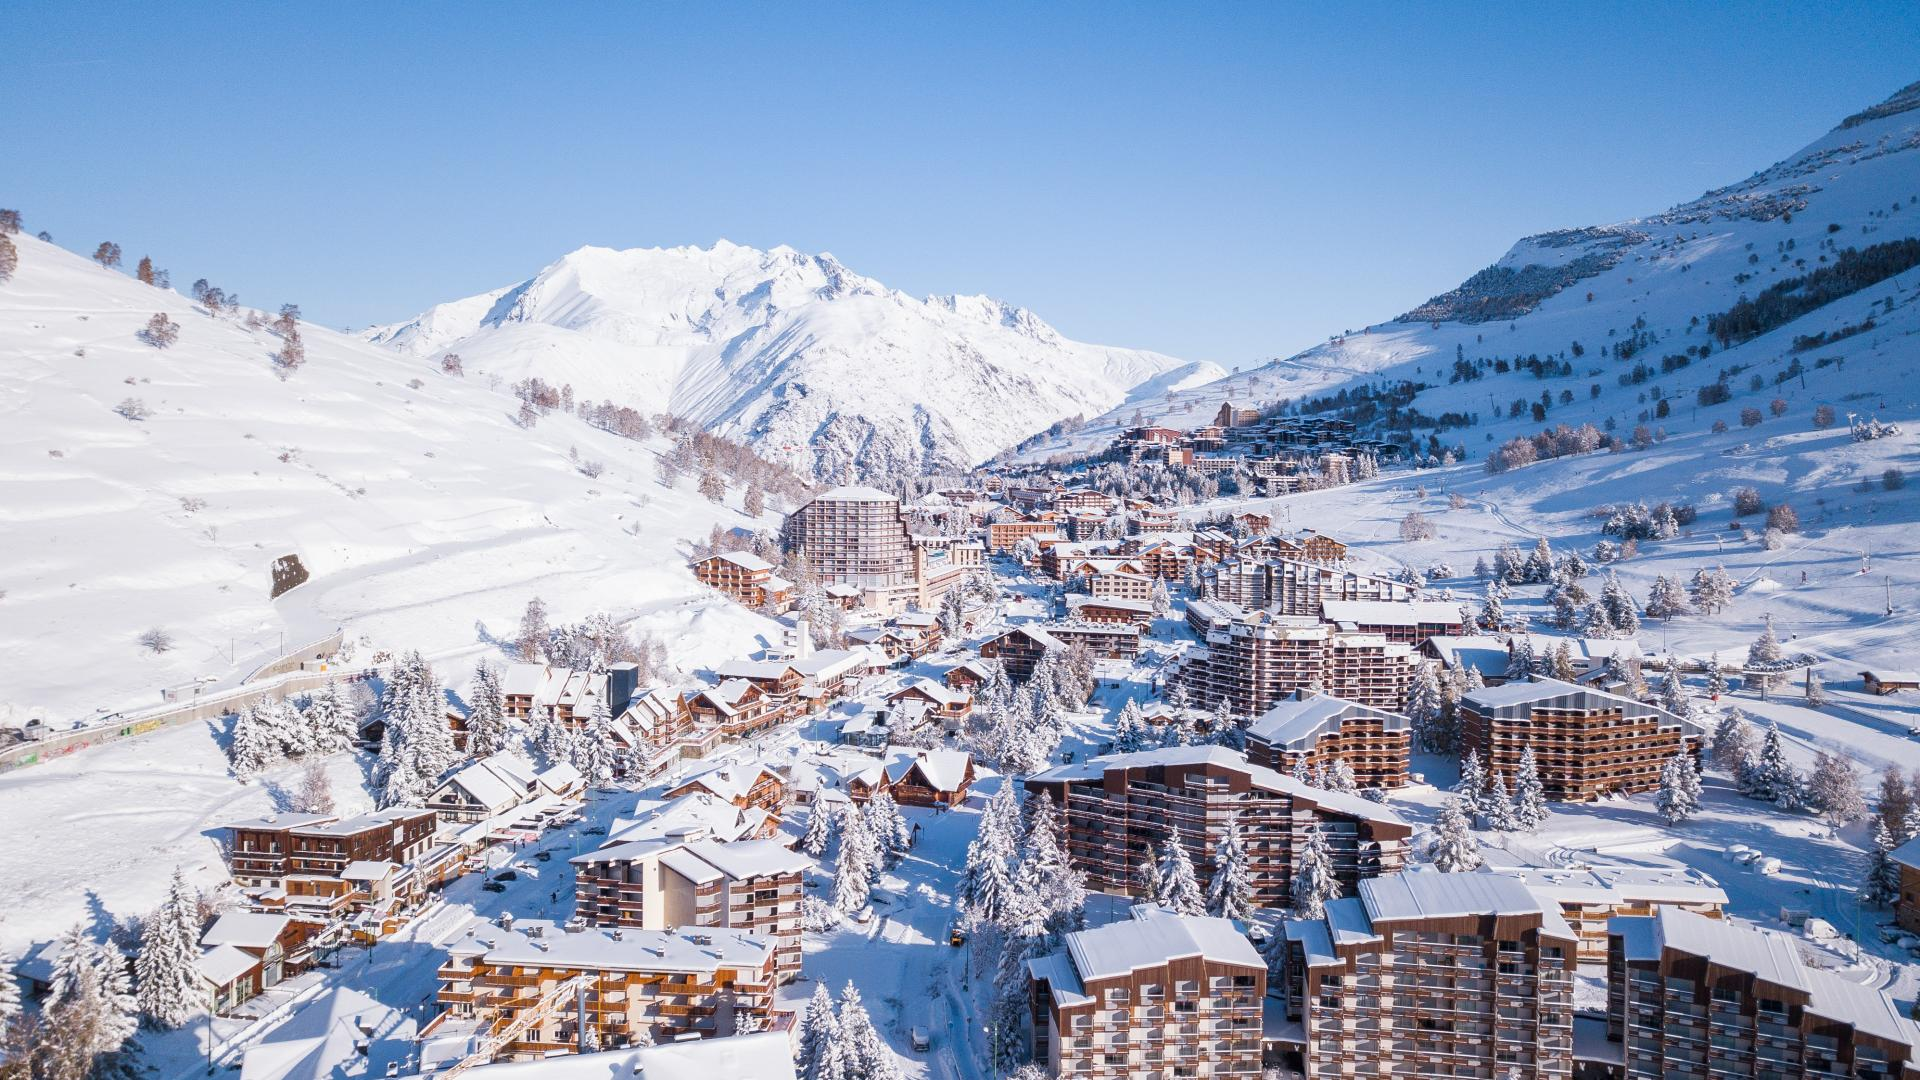
\includegraphics[scale=0.115]{alpes.jpg}
            }
            \only<5-6>{
              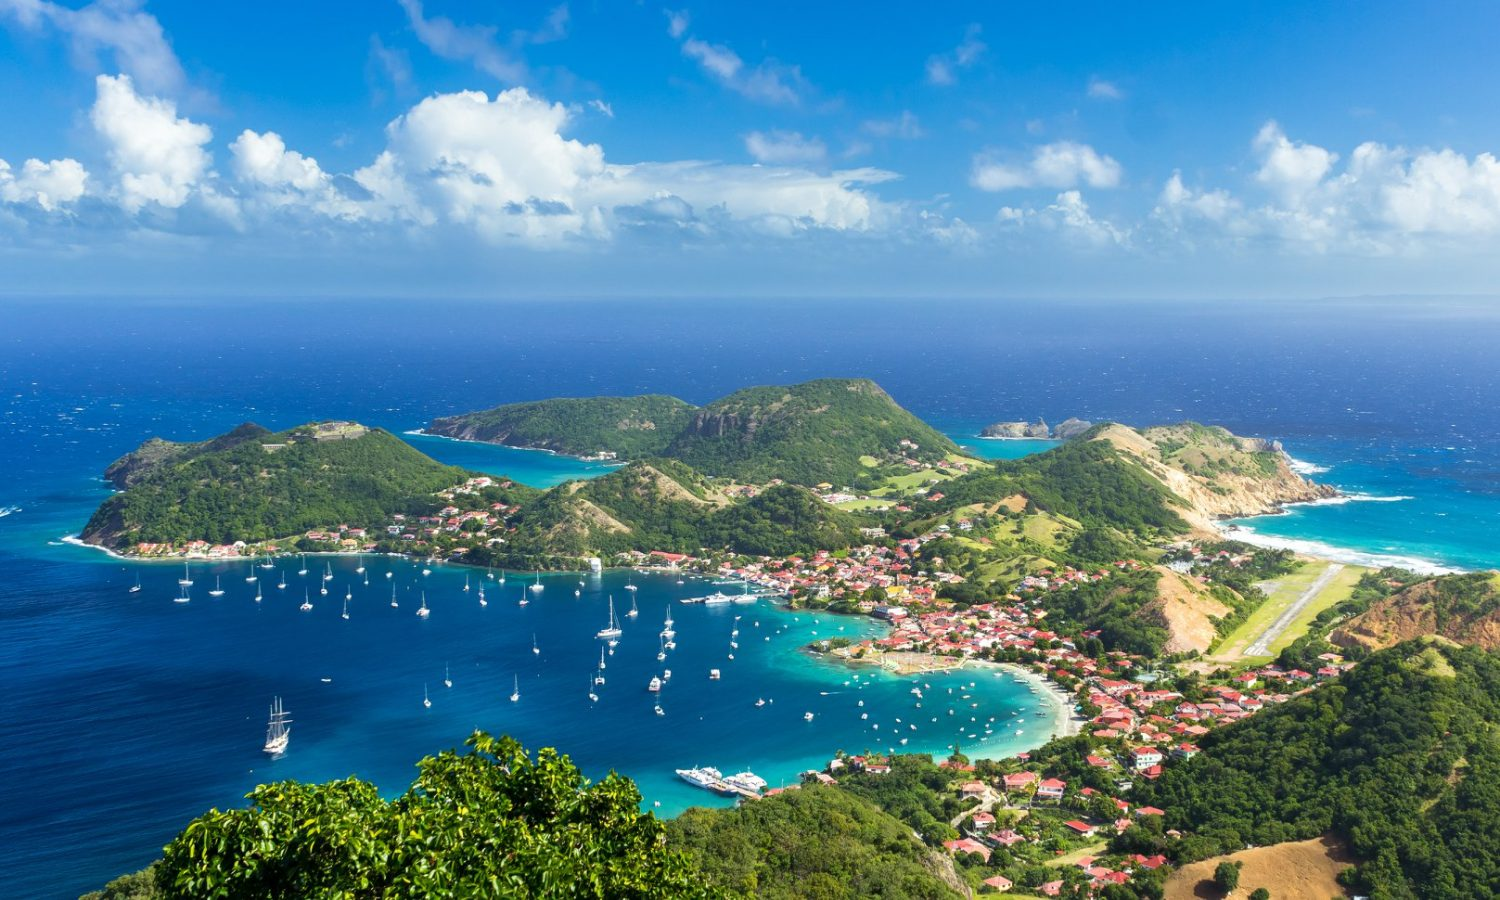
\includegraphics[scale=0.145]{guadeloupe.jpg}
            }
            \only<7-8>{
              \includegraphics[scale=0.125]{mexique_musée.jpg} \\
              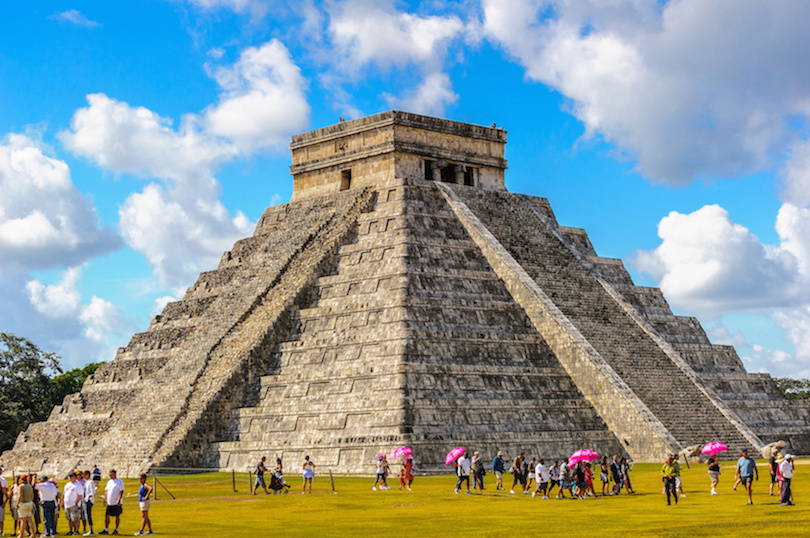
\includegraphics[scale=0.175]{mexique_pyramide.jpg}
            }
          \end{center}
        \end{minipage}
    \end{columns}
  \end{frame}

  \begin{frame}{}
    \begin{center}
      \Large Quiz
    \end{center}
  \end{frame}

  \begin{frame}{Boule de cristal}
    \begin{columns}
      \column{0.4\textwidth}
        \begin{center}
          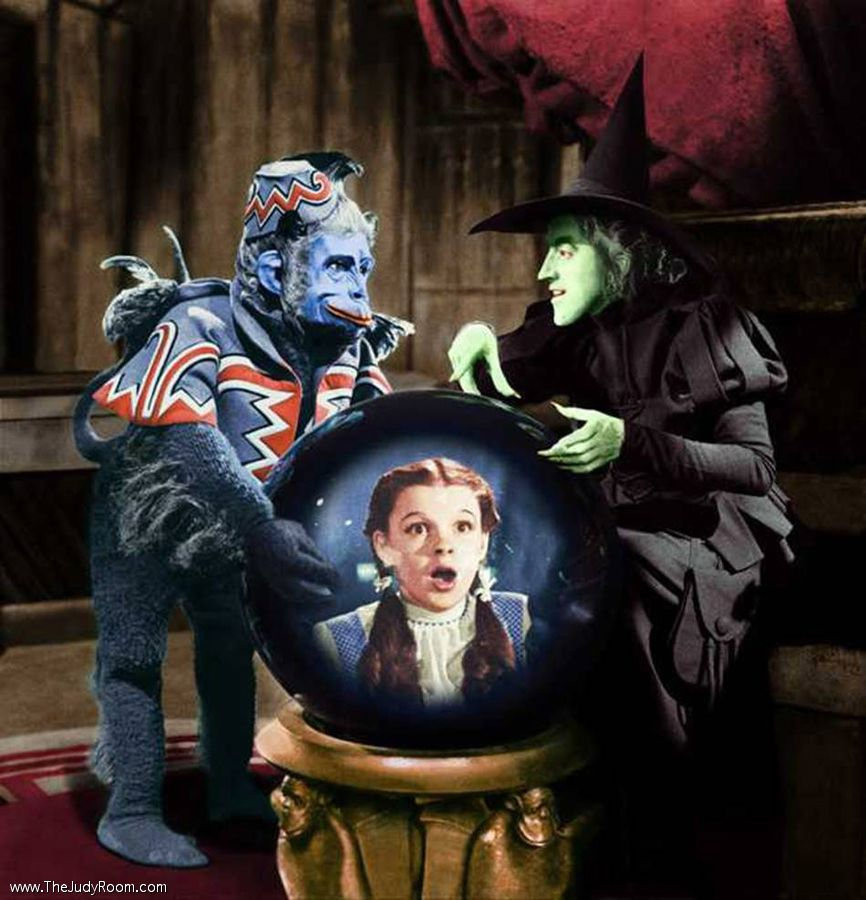
\includegraphics[scale=0.15]{boule_cristal.jpg}
        \end{center}
      \column{0.6\textwidth}
        \scriptsize
        Avec un/e partenaire, imaginez que vous allez chez une voyante.
        Tirez \gloss{draw} des conclusions de ses prédictions, et comparez vos conclusions.
        \begin{description}
          \item[] \textbf{Modèle:} \textit{Beaucoup d'argent passera entre tes mains.}
          \item[E1:] Alors, je serai très riche.
          \item[E2:] Ou alors, je travaillerai dans une banque.
        \end{description}
        \begin{enumerate}
          \item Tu travailleras beaucoup à cause du travail.
          \item Il y aura beaucoup d'enfants dans ta vie.
          \item Tu seras devant une grande maison.
          \item Tu seras en compagnie d'une belle femme ou d'un bel homme.
          \item Vous aurez beaucoup d'amis, vous deux.
          \item Vous serez très célèbre, vous deux.
        \end{enumerate}
    \end{columns}
  \end{frame}

  \begin{frame}{}
    \begin{center}
      \Large Questions?
    \end{center}
  \end{frame}
\end{document}
